\documentclass[a4paper,14pt]{article}
\usepackage[utf8]{inputenc}
\usepackage[russian]{babel}
\usepackage{geometry} % Меняем поля страницы
\geometry{left=2.5cm}% левое поле
\geometry{right=1cm}% правое поле
\geometry{top=2cm}% верхнее поле
\geometry{bottom=2cm}% нижнее поле
\setlength{\parindent}{1cm}
\parindent=1.25cm		% абзацный отступ
\linespread{1.3}     % межстрочный интервал
\tolerance=2000
\usepackage{amsmath,amssymb,graphicx,misccorr,indentfirst}
\renewcommand{\rmdefault}{cmr}
\usepackage{amsmath}
\usepackage[labelsep=period]{caption}
\usepackage{fancyhdr}
\usepackage{ragged2e}
\pagestyle{fancy}
\fancyhf{} % clear all header and footer fields
\fancyhead[C]{\thepage}
\renewcommand{\headrulewidth}{0pt}
\renewcommand{\footrulewidth}{0pt}
% redefinition of the plain style:
\fancypagestyle{plain}{%
\fancyhf{} % clear all header and footer fields
\fancyhead[C]{\thepage}
\renewcommand{\headrulewidth}{0pt}
\renewcommand{\footrulewidth}{0pt}}
\captionsetup[table]{justification=raggedright,singlelinecheck=off}
\DeclareUnicodeCharacter{2212}{-} 

\begin{document}
\begin{titlepage}
\begin{center}
    \large
    ФЕДЕРАЛЬНОЕ ГОСУДАРСТВЕННОЕ БЮДЖЕТНОЕ ОБРАЗОВАТЕЛЬНОЕ УЧРЕЖДЕНИЕ ВЫСШЕГО ОБРАЗОВАНИЯ «МОСКОВСКИЙ ГОСУДАРСТВЕННЫЙ УНИВЕРСИТЕТ ИМЕНИ М.В.ЛОМОНОСОВА»
     
    \textbf{Физический факультет}\\
    \vspace{4cm}
    \textsc{\Large Отчет по практическому заданию №1}\\[5mm]
    {\LARGE Основы математического моделирования.}
\end{center}
\vspace{7cm}
\null
\begin{flushright}
\normalsize студента 327 группы
\\Иванова Ивана Ивановича
\end{flushright}
\vfill
\begin{center}
\textbf{Москва - 2021}
\end{center}
\end{titlepage}


\section{Постановка задачи.}
Используя схему бегущего счёта и итерационные методы, решить задачу:

\begin{equation*}
\begin{cases}
   \frac{\partial u}{\partial t} - \frac{1}{1+u} \frac{\partial u}{\partial x}=0, \qquad -1\leqslant x<0\\
   u(x,0)=\cos(\frac{\pi x}{2})\\
   u(0,t)= \exp(-t)
 \end{cases}
\end{equation*}


\section{Характеристики уравнения.}
Исследуем существование единственного решения в заданной области, т.е.
определим, претерпевает ли решение разрыв в области $D: {x \in [−1,0), t \in (0, T)}$. Для этого составим уравнение характеристик и исследуем их на наличие пересечений в заданной области поиска решения. Если пересечения будут, то это означает, что в этой точке существует столько решений, сколько характеристик в ней пересекаются. Если пересечений не будет, то в данной области существует единственное решение поставленной задачи.

$$\frac{d t}{1}=-(1+u)\frac{d x}{1}=\frac{d u}{0}$$

\noindent получаем, что $u = const = u(x_0, t_0)$ и получаем уравнение характеристики, на которой $u$ является константой:

$$\frac{d x}{d t}=-\frac{1}{1+u}$$

\noindent Проинтегрирую это уравнение: $t-t_0 = -(1+u)(x-x_0)$

Учитывая начальные и граничные условия, получим, что характеристики будут иметь следующий вид:

$t = -(1+cos(\frac{\pi x_0}{2}))(x-x_0)$,\qquad при $t_0=0$ и различных $x_0$
\vspace{0.4 cm}

$t = t_0 - (1+\exp(-t_0))x$,\qquad при $x_0=0$ и различных $t_0$

\vspace{0.5 cm}
Эти характеристики и будем проверять на наличие пересечений в области поиска решения. Из графиков, представленных ниже, видно, что в рассматриваемой области $D: {x \in [−1,0), t \in (0, T)}$ характеристики не пересекаются, следовательно, нет опрокидывания волны. Решение на нашем интервале определено однозначно.


\begin{figure}[h!]
\centering
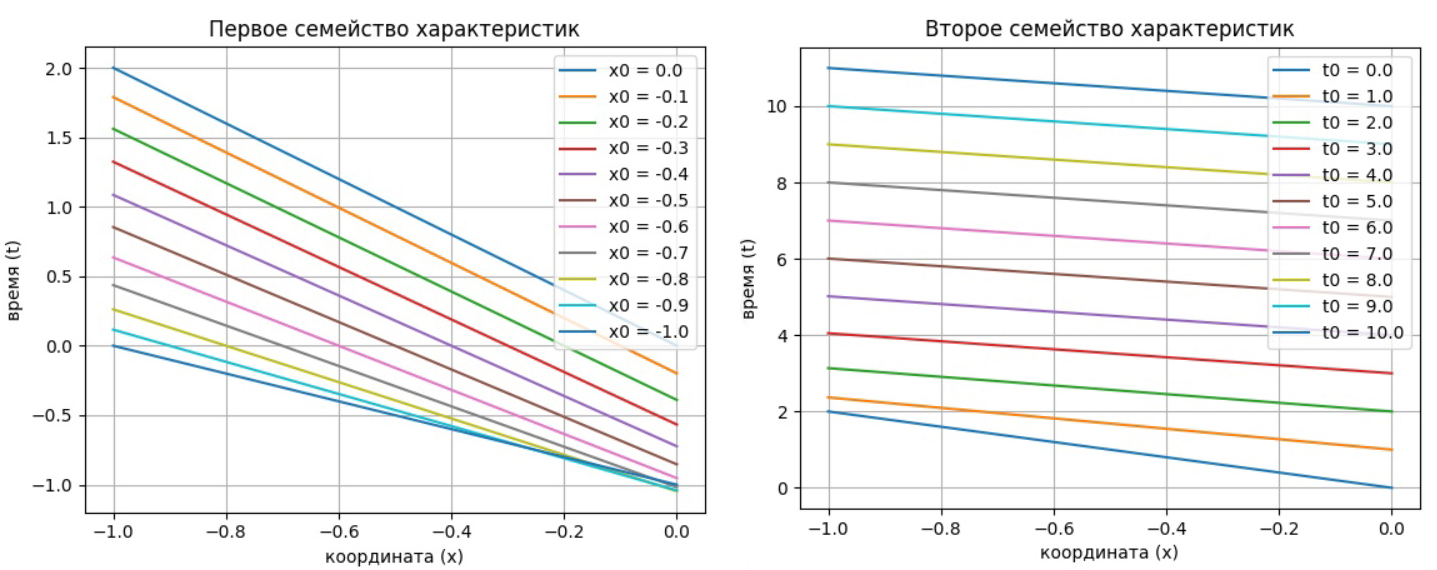
\includegraphics[scale=0.35]{характеристики.jpg}
\caption{\label{pic1}Характеристики уравнения}
\end{figure}

Теперь найду точное решение поставленной задачи в неявном виде методом характеристик. Выберу некоторое $x^*$. Из начальных условий имеем, что $u(x^*,0)=\cos(\frac{\pi x^*}{2})$. На характеристике $u(x^*,t)=\cos(\frac{\pi x^*}{2})=const$. Тогда получим решение уравнения в виде:

\begin{equation*}
\begin{cases}
   x = x^* - \frac{1}{1+\cos(\frac{\pi x^*}{2})}t\\
   u(x,t)=\cos(\frac{\pi x^*}{2})
 \end{cases}
\end{equation*}


\section{Метод решения.}
Перейдем теперь к построению разностной схемы. Введем равномерную сетку:

$x_i=nh,\qquad n = 0,...,N, \qquad h = -\frac{1}{N}, \qquad  t_j=\tau m, \qquad m = 0,...,M \qquad \tau=\frac{1}{M}$

Здесь N – число узлов по х, а M – число узлов по t. Перепишем исходное уравнение в виде:

$$\frac{\partial u}{\partial t} - \frac{\partial (\ln(1+u))}{\partial x}=0$$

\noindent Обозначим $f(u) = -\ln(1+u)$

Составлять схему будем методом разностной аппроксимации. Введем сеточную функцию $y_{n,m}$ следующим образом: 

$$y_{n,m} = u(x_n,t_m)=y_n, \qquad f(y_{n,m})=f_n$$

Для простоты обозначу значения функций на $m+1$ слое как: $y_{n,m+1} = \hat{y_n}, \qquad f(y_{n,m+1})=\hat{f_n}$

Для решения уравнения на сетке используется четырехточечный шаблон, поскольку при
использовании такого шаблона разностная схема безусловно устойчива, и она имеет
порядок аппроксимации $O(\tau^2 + h^2)$. Трехточечные шаблоны не применимы, так как коэффициент при $\frac{\partial u}{\partial x}$: $c<0$. Можно показать, что безусловная устойчивость будет отсутствовать. 

Разностная аппроксимация уравнения в точке $(x_n + \frac{h}{2}, t_m + \frac{\tau}{2})$ имеет вид:

\begin{equation*}
\begin{cases}
   \frac{\hat{y}_n-y_n+\hat{y}_{n+1}-y_{n+1}}{2 \tau} + \frac{f_{n+1}-f_n+\hat{f}_{n+1}-\hat{f}_n}{2 h}=0\\
   y_{n, 0}=\cos(\frac{\pi x_n}{2})\\
   y(0,m)= \exp(-t_m)
 \end{cases}
\end{equation*}

\begin{figure}[h!]
\centering
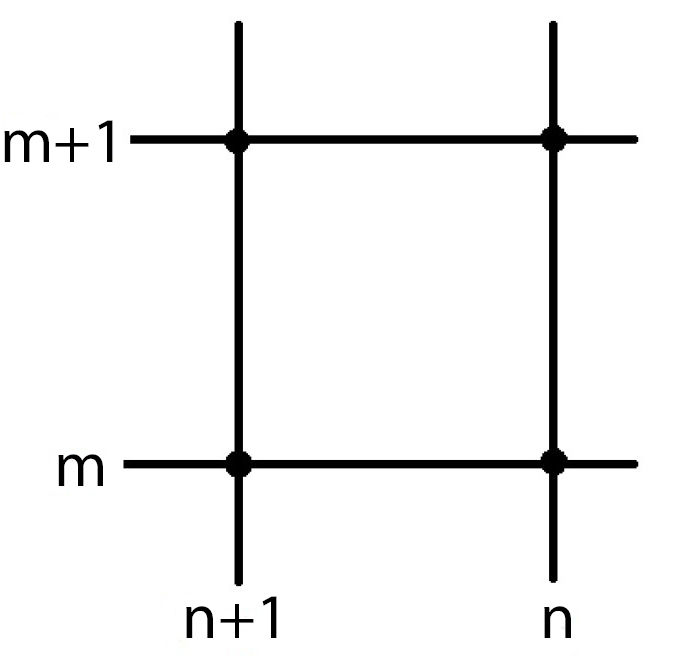
\includegraphics[scale=0.4]{сетка.jpg}
\caption{\label{pic2}Четырехточечный шаблон}
\end{figure}

Данную задачу будем решать при помощи схемы бегущего счета. Значение сеточной функции: $y_{n+1,m+1}$ неизвестно. Считая значения на m-ом слое известным, найдем решение на (m+1) слое. В результате чего можно по начальному и граничному условиям найти решение для любого последующего момента времени. В итоге получим уравнение относительно $\hat{y}_{n+1}$, которое будем решать итерационным методом Ньютона.

$$g(\hat{y}_{n+1})=\frac{\hat{y}_n-y_n+\hat{y}_{n+1}-y_{n+1}}{2 \tau} - \frac{\ln(y_{n+1})-\ln(y_n)+\ln(\hat{y}_{n+1})-\ln(\hat{y}_n)}{2 h}=0$$
$$g'(\hat{y}_{n+1})=\frac{1}{2 \tau}-\frac{1}{2h(1+\hat{y}_{n+1})}$$

\noindent Пусть известно некоторое приближение $\hat{y}_{n+1}^{(k)}$ к корню $\hat{y}_{n+1}$, тогда уравнение примет вид:
$$g(\hat{y}_{n+1}^{(k)}+\Delta \hat{y}_{n+1}^{(k)})=0, \qquad \Delta \hat{y}_{n+1}^{(k)} = \hat{y}_{n+1} - \hat{y}_{n+1}^{(k)}$$

\noindent Разложим уравнение в ряд Тейлора, оставляя только член первого порядка малости, получим:
$$\Delta \hat{y}_{n+1}^{(k)} = - \frac{g(\hat{y}_{n+1}^{(k)})}{g'(\hat{y}_{n+1}^{(k)})}$$

\noindent В итоге получим формулу:

$$\hat{y}_{n+1}^{(k+1)}= \hat{y}_{n+1}^{(k)}-\frac{g(\hat{y}_{n+1}^{(k)})}{g'(\hat{y}_{n+1}^{(k)})}$$

\noindent Процесс останавливается при достижении заданной точности (невязки) $\varepsilon: |\hat{y}_{n+1}^{(k)}-\hat{y}_{n+1}^{(k-1)}|<\varepsilon$ или при достижении 10000 итераций. Тогда $\hat{y}_{n+1}=\hat{y}_{n+1}^{(k)}$

\section{Проверка сходимости по спектральному критерию Неймана.}
Введу функцию: $C(u)= -\frac{1}{1+u}$.

Выберем какую-нибудь произвольную точку (xo,t0). Зафиксируем функцию перед $\frac{\partial u}{\partial x}$, возьмём её равной $C$. Тогда разностная схема будет иметь вид:
$$\frac{\hat{y}_n-y_n+\hat{y}_{n+1}-y_{n+1}}{2 \tau} + C\frac{y_{n+1}-y_n+\hat{y}_{n+1}-\hat{y}_n}{2 h}=0\\$$

\noindent Подставляем решение в виде: $y_{n, m} = \lambda^m e^{i \omega n}$. Выражая $\lambda$ из этого уравнения получаем:

$$\lambda = \frac{h(1+e^{i \omega})+C \tau (e^{i \omega}-1)}{h(1+e^{i \omega}) - C \tau(e^{i \omega}-1)}$$

$$|\lambda| = |\frac{\cos(\frac{\omega}{2})+\frac{i c \tau}{h}\sin(\frac{\omega)}{2})}{\cos(\frac{\omega}{2})-\frac{i c \tau}{h}\sin(\frac{\omega)}{2})}|=1$$

Из этого выражения видно, что условие $|\lambda(\omega)|\leqslant 1$ выполнено для любых значений шага по времени и координате, следовательно, спектральный критерий Неймана также выполнен для любых $\tau$ и $h$. Необходимое условие устойчивости выполнено. 

\section{Достаточное условие сходимости.}
Запишу разностную схему в следующем виде: 
\begin{equation*}
\begin{cases}
   \hat{y}_{n+1}(1 - \frac{C \tau}{h})+\hat{y}_n(1 + \frac{C \tau}{h})= y_n (1 - \frac{C \tau}{h})+ y_{n+1}(1 + \frac{C \tau}{h}) + \tau (\hat{f}_{n} + f_{n+1}) \\
   y_{n,0}=\phi_n
 \end{cases}
\end{equation*}

Мажорантно оценим левую часть уравнения. Получаем:

$$|\hat{y}_{n+1}|(1 - \frac{C \tau}{h})+|\hat{y}_n|(1 + \frac{C \tau}{h}) \leqslant |y_n| (1 - \frac{C \tau}{h})+ |y_{n+1}|(1 + \frac{C \tau}{h}) + \tau (|\hat{f}_{n}| + |f_{n+1}|)  \leqslant 2\|y_m\|+2 \tau\|f\|$$

\noindent где, $\|f\|= \max\limits_{n,m}|f_{n,m}|$, а $\|y_m\|= \max\limits_{n}|y_{n,m}|$. Отсюда получаем, что $\|y_{m+1}\| \leqslant \|y_m\|+ \tau\|f\|$.

Следовательно, $\|y_{m}\| \leqslant \|y_0\|+ m\tau\|f\| \leqslant \|\phi\| + T\|f\|$, где $T$ - величина интервала времени, на котором мы ищем решение. Эта оценка,
по определению, означает устойчивость решения задачи по начальным данным и правой части. 

\section{Геометрический критерий сходимости.}
Рассмотрим шаблон разностной схемы. Имеется простой геометрический критерий, позволяющий установить условия устойчивости той или иной схемы бегущего счета по виду шаблона. А именно, на каждом шаге вычисления по любой из рассматриваемых схем, в одной из точек шаблона разностная функция ищется, а в остальных уже известна. Проведем характеристику уравнения из точки, где решение ищется. Если шаги и h выбраны так, что эта характеристика пересекает отрезок соединяющий точки шаблона, в которых решение известно, то схема будет устойчивой. Если же характеристика проходит мимо такого отрезка, то неустойчивой.

\begin{figure}[h!]
\centering
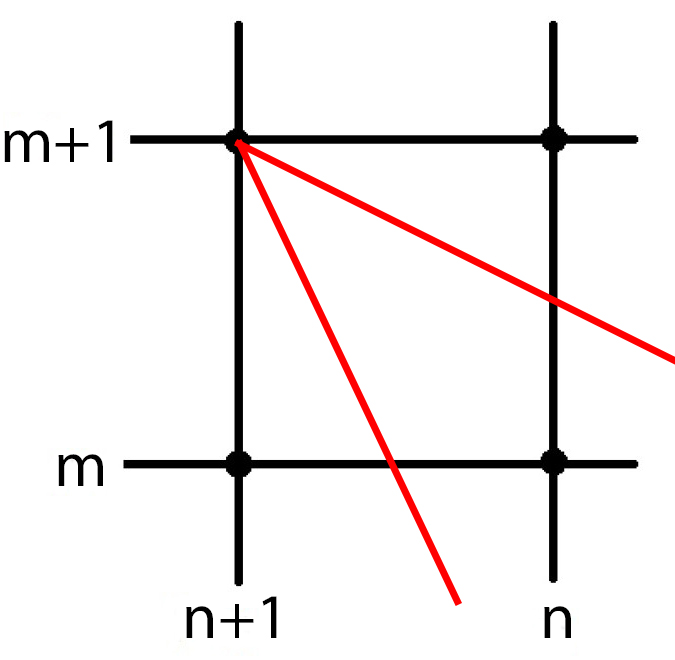
\includegraphics[scale=0.4]{сетка_сход.jpg}
\caption{\label{pic3}Геометрический критерий сходимости.}
\end{figure}

По рисунку видно, что характеристика всегда пересекает отрезок, соединяющий точки, в которых решение известно, при любых выбранных шагах сетки. Таким образом, схема является безусловно устойчивой.

\section{Порядок аппроксимации разностной схемы.}
Для аппроксимации используется четырехточечный шаблон – схема с симметричными производными. Вычислим порядок аппроксимации (невязку) для этого шаблона.
Для этого разложим функции в ряд Тейлора в середине квадрата, т.е. в точке $(x_n + \frac{h}{2}, t_m + \frac{\tau}{2})$.

$$y_{n+1}^{m+1} = y_{n+0.5}^{m + 0.5} + (\frac{\partial}{\partial t}\frac{\tau}{2}+\frac{\partial}{\partial x}\frac{h}{2})y+
\frac{1}{2}(\frac{\partial}{\partial t}\frac{\tau}{2}+\frac{\partial }{\partial x}\frac{h}{2})^2 y + 
\frac{1}{6}(\frac{\partial}{\partial t}\frac{\tau}{2}+\frac{\partial}{\partial x}\frac{h}{2})^3 y +...$$

$$y_{n}^{m+1} = y_{n+0.5}^{m + 0.5} + (\frac{\partial}{\partial t}\frac{\tau}{2}-\frac{\partial}{\partial x}\frac{h}{2})y+
\frac{1}{2}(\frac{\partial}{\partial t}\frac{\tau}{2}-\frac{\partial }{\partial x}\frac{h}{2})^2 y + 
\frac{1}{6}(\frac{\partial}{\partial t}\frac{\tau}{2}-\frac{\partial}{\partial x}\frac{h}{2})^3 y +...$$

$$y_{n+1}^{m} = y_{n+0.5}^{m + 0.5} + (-\frac{\partial}{\partial t}\frac{\tau}{2}+\frac{\partial}{\partial x}\frac{h}{2})y+
\frac{1}{2}(-\frac{\partial}{\partial t}\frac{\tau}{2}+\frac{\partial }{\partial x}\frac{h}{2})^2 y + 
\frac{1}{6}(-\frac{\partial}{\partial t}\frac{\tau}{2}+\frac{\partial}{\partial x}\frac{h}{2})^3 y +...$$

$$y_{n}^{m} = y_{n+0.5}^{m + 0.5} - (\frac{\partial}{\partial t}\frac{\tau}{2}+\frac{\partial}{\partial x}\frac{h}{2})y+
\frac{1}{2}(\frac{\partial}{\partial t}\frac{\tau}{2}+\frac{\partial }{\partial x}\frac{h}{2})^2 y - 
\frac{1}{6}(\frac{\partial}{\partial t}\frac{\tau}{2}+\frac{\partial}{\partial x}\frac{h}{2})^3 y +...$$


Приводя подобные слагаемые, имеем с точностью до членов следующего порядка малости:

$$\frac{\hat{y}_n-y_n+\hat{y}_{n+1}-y_{n+1}}{2 \tau} = \frac{\partial y}{\partial t} + \frac{1}{24}\tau^2 y_{ttt} + \frac{1}{8} h^2 y_{txx}$$


$$\frac{\hat{c}_n-c_n+\hat{c}_{n+1}-c_{n+1}}{2 h} = \frac{\partial c}{\partial x} + \frac{1}{8} \tau^2  c_{xtt} + \frac{1}{24} h^2 c_{xxx}$$

Таким образом, разностная схема аппроксимирует задачу с вторым порядком малости как по пространственной координате, так и по времени.

\section{Результаты.}
В результате выполнения программы получены следующие графики:

\begin{figure}[h!]
\centering
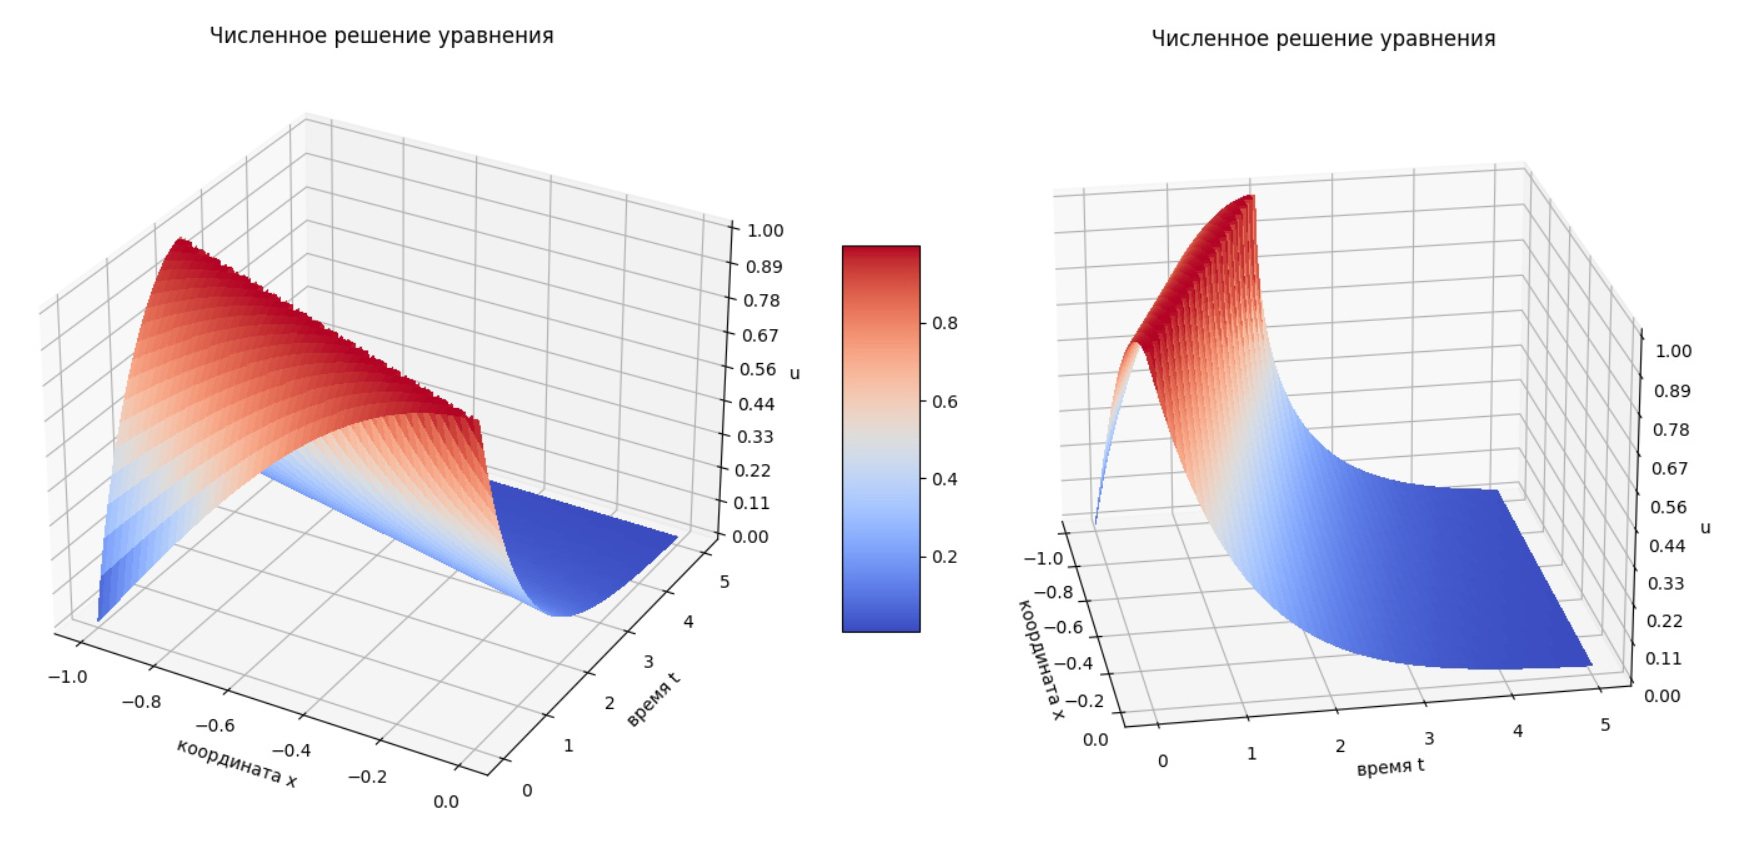
\includegraphics[scale=0.3]{решение.jpg}
\caption{\label{pic4}}
\end{figure}

Модуль разности рассчитывался между решениями с записанным на графике (рис.\ref{pic5}) шагом по времени и координате и вдвое большим. Видно, что чем меньше шаг, тем меньше модуль разности между решениями, что подтверждает сходимость.

\begin{figure}[h!]
\centering
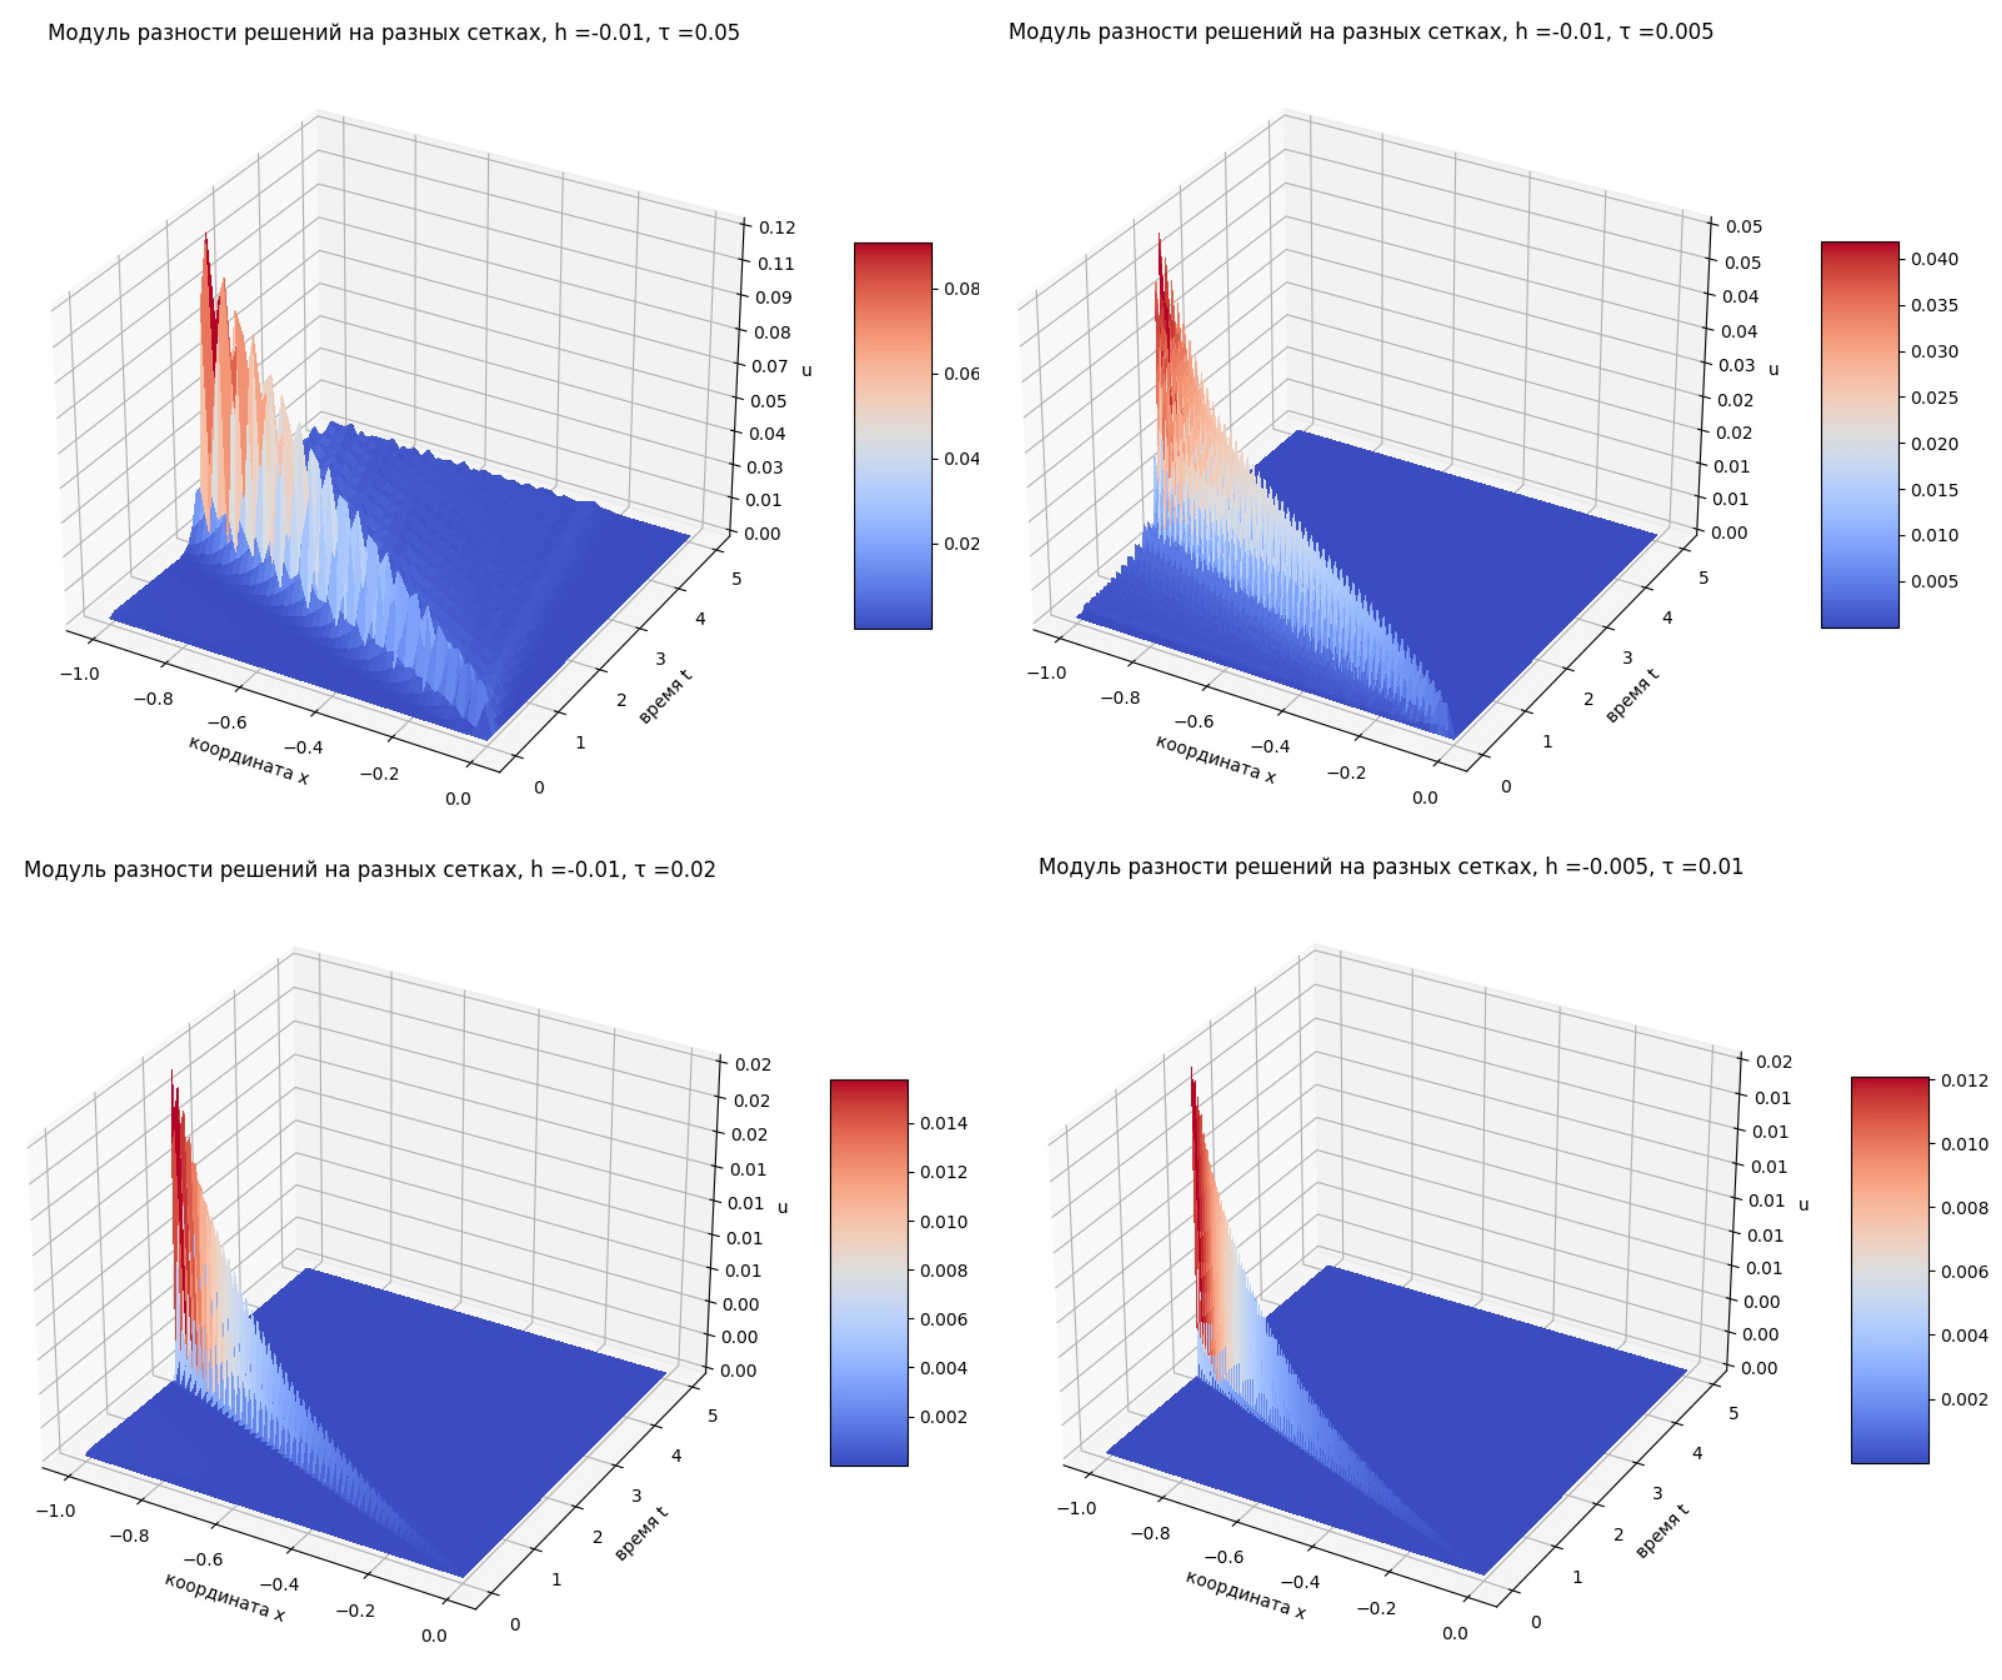
\includegraphics[scale=0.25]{погрешность.jpg}
\caption{\label{pic5}}
\end{figure}

Как видно из рисунка \ref{pic6} граничные и начальные условия заданы верно.

\begin{figure}[h!]
\centering
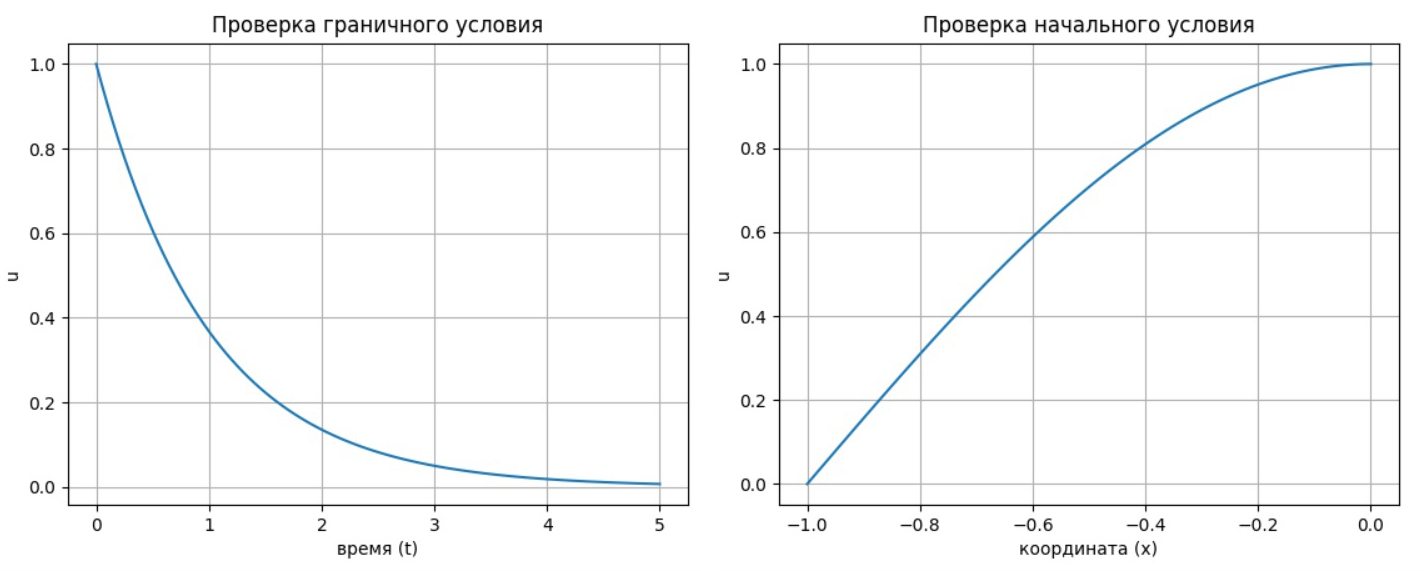
\includegraphics[scale=0.35]{ГУНУ.jpg}
\caption{\label{pic6}}
\end{figure}

На рисунках \ref{pic7} и \ref{pic8} проилюстрирована сходимость при разных шагах по времени и координате.

\begin{figure}[h!]
\centering
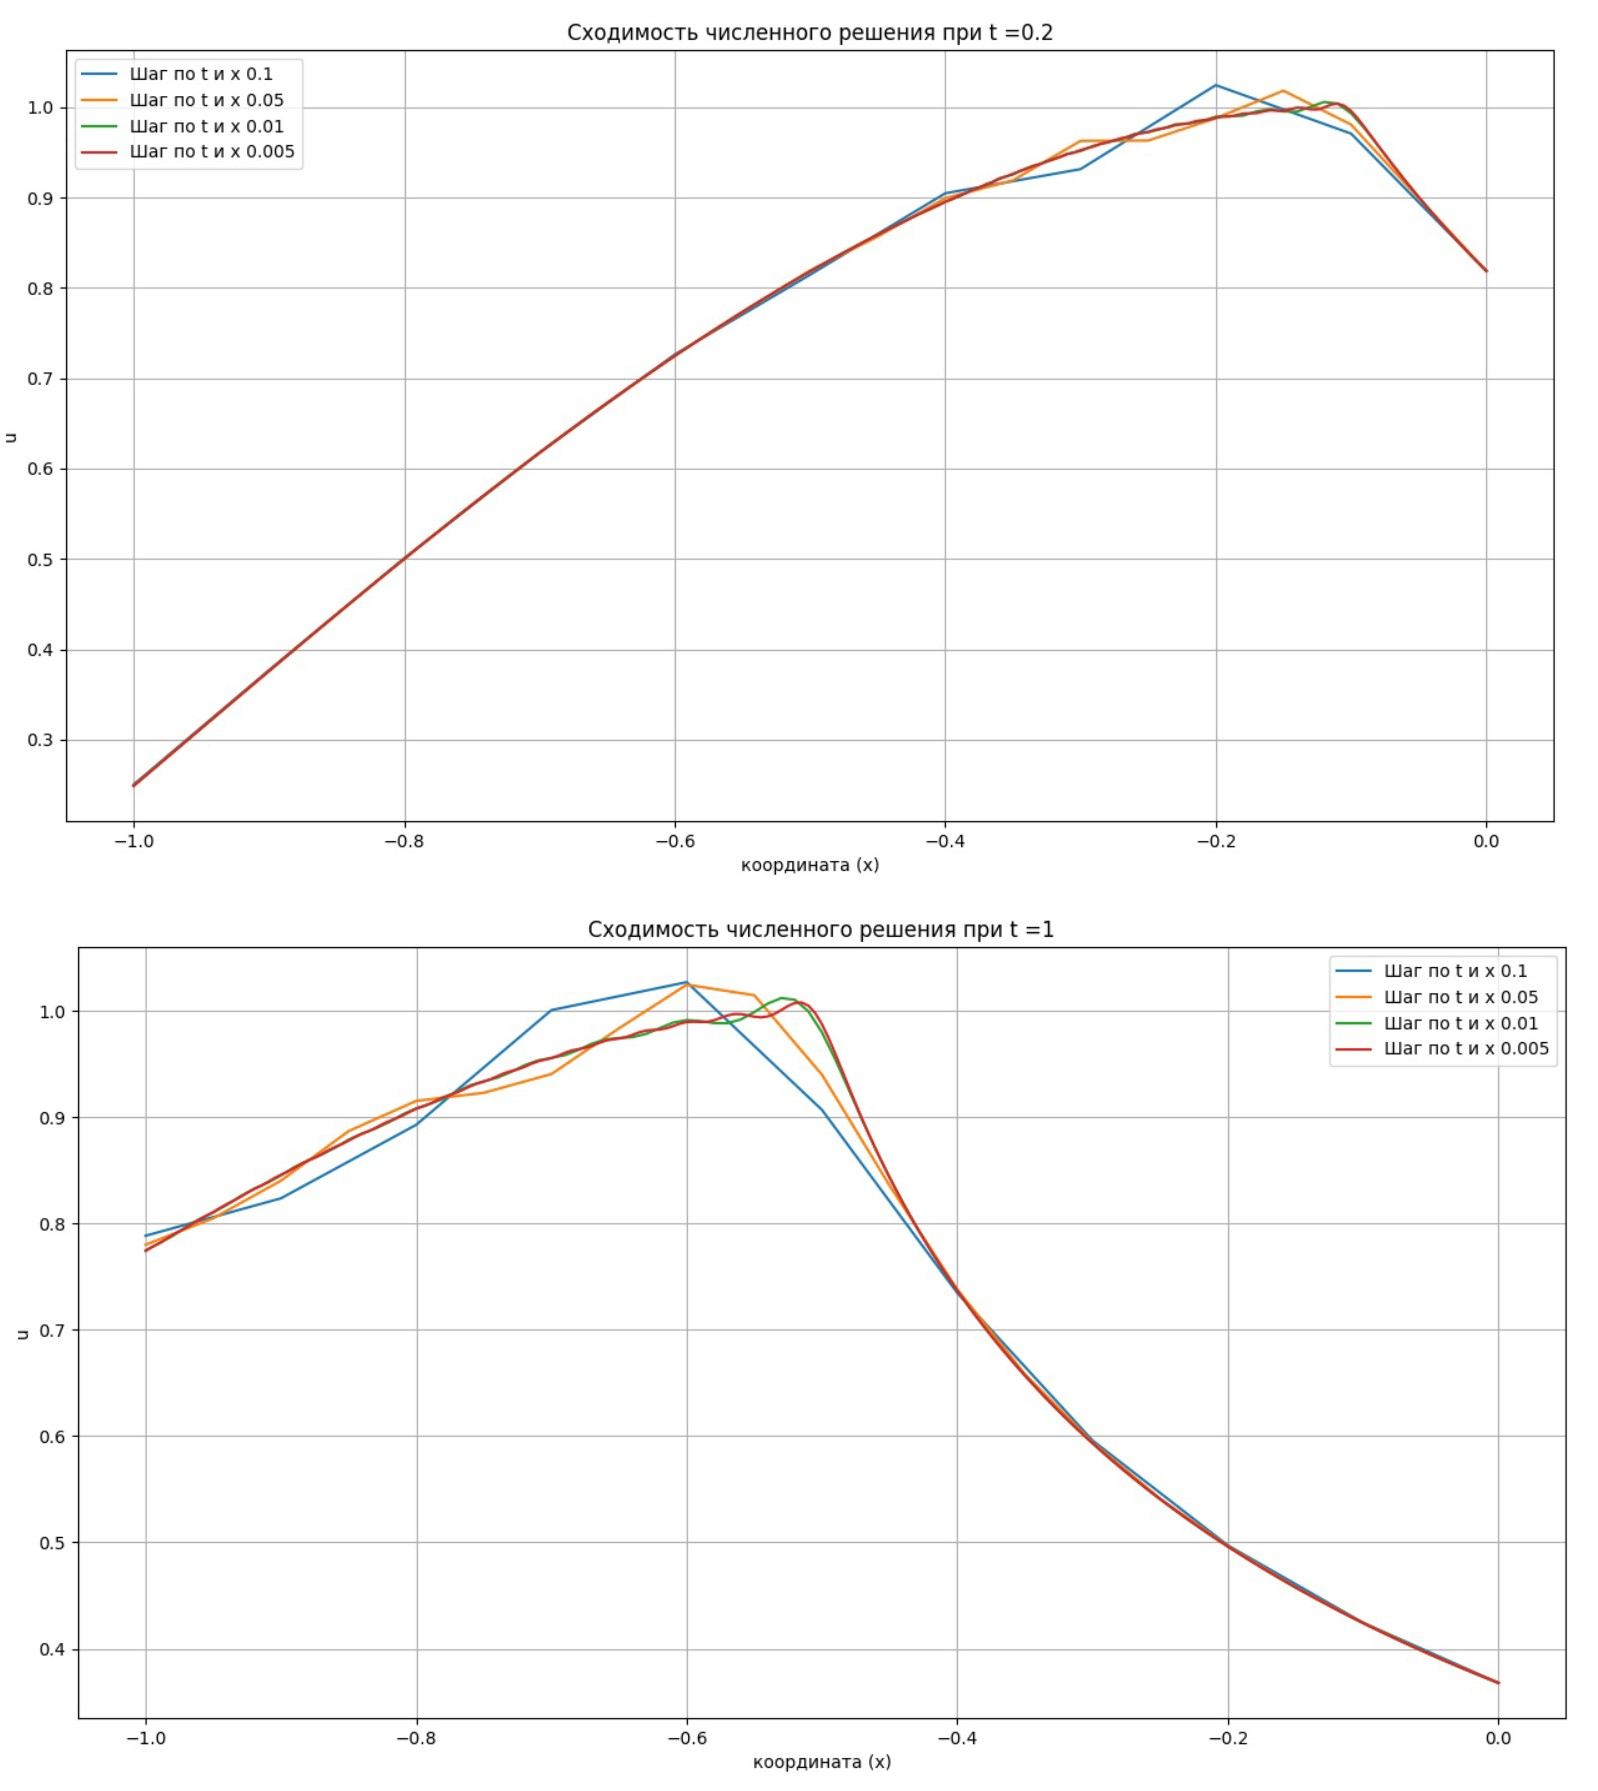
\includegraphics[scale=0.3]{сходимость1.jpg}
\caption{\label{pic7}}
\end{figure}

\begin{figure}[h!]
\centering
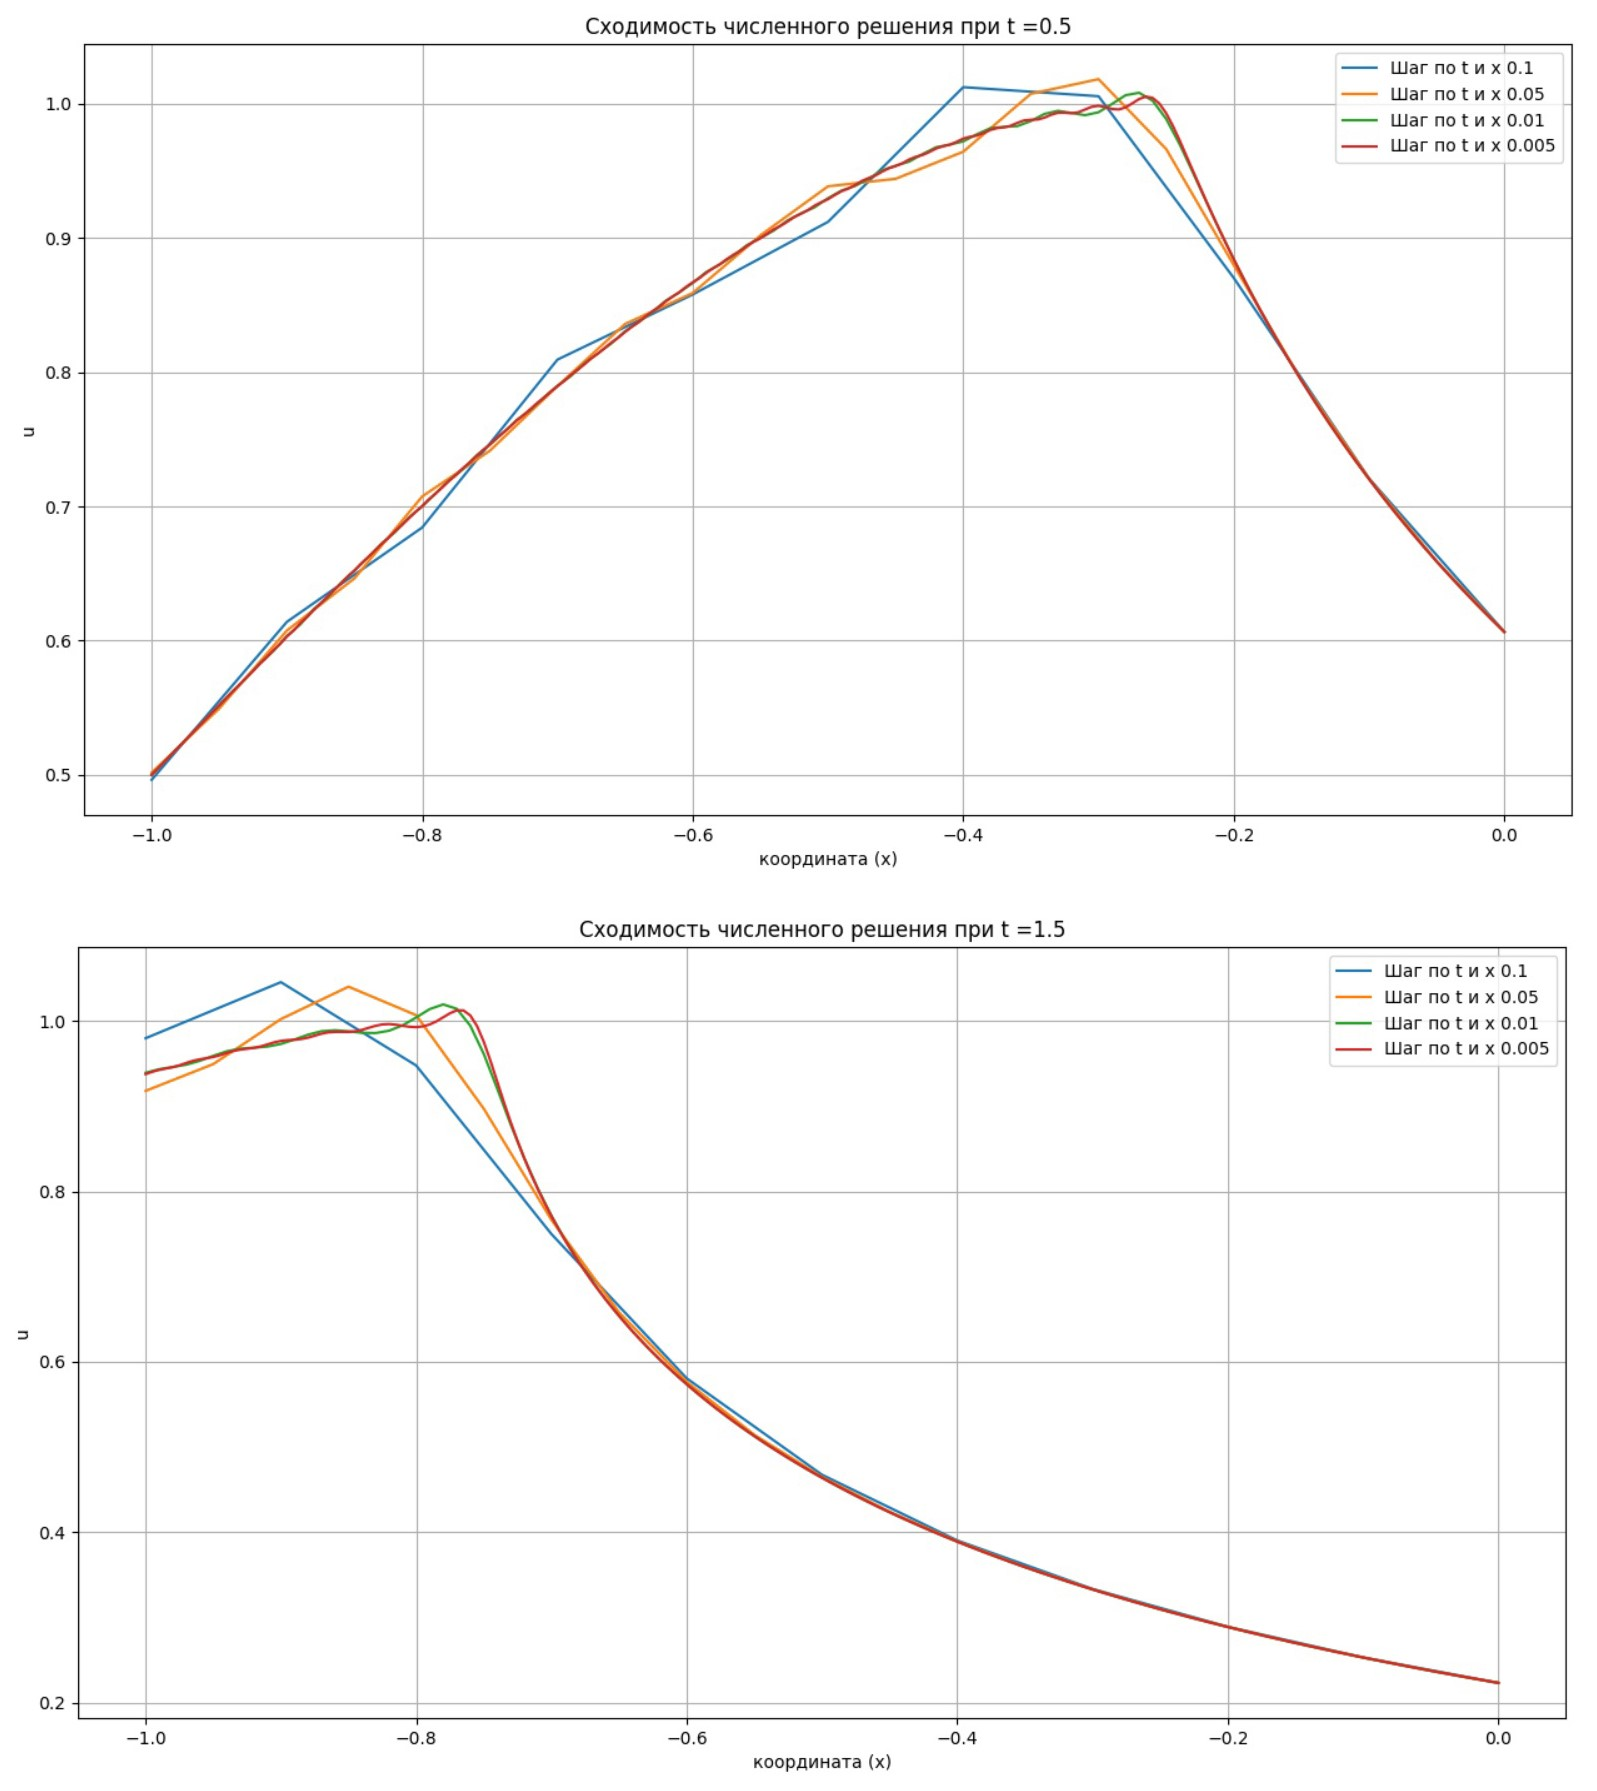
\includegraphics[scale=0.3]{сходимость2.jpg}
\caption{\label{pic8}}
\end{figure}

\end{document}
